\chapter{REFERENCIAL TEÓRICO}
\label{chap:LR}

\section{Exercícios de Força e Biomecânica}

O treinamento de força, também denominado treinamento resistido, é uma prática consolidada para a melhoria da aptidão física, do desempenho esportivo e da saúde geral da população. Ele consiste na realização de exercícios em que a musculatura esquelética atua contra uma resistência externa, podendo ser pesos livres, máquinas, elásticos ou o próprio peso corporal. A manipulação de variáveis como intensidade, volume, frequência, intervalos e cadência possibilita diferentes adaptações fisiológicas e neuromusculares \cite{william-j-kraemer-fundamentos-2021,murer-treinamento-2022}.

Diversos estudos confirmam os benefícios do treinamento de força, entre eles: aumento de força e potência muscular, hipertrofia, melhora da densidade mineral óssea, auxílio na perda de gordura, além de impactos positivos na saúde cardiovascular, metabólica e mental \cite{murer-treinamento-2022,thiago-da-silva-machado-treinamento-nodate,pinto-aplicacao-2023}. Em populações idosas, o treinamento resistido é ainda mais relevante, pois atua na preservação da massa muscular e da funcionalidade, reduzindo o risco de quedas e promovendo maior independência \cite{murer-treinamento-2022}.

No contexto da prática, diferentes equipamentos podem ser empregados. Os pesos livres (halteres e barras) são amplamente utilizados por sua versatilidade e por possibilitarem maior recrutamento de músculos estabilizadores, além de permitirem variações de movimento mais próximas da realidade funcional. Contudo, exigem maior controle motor e conhecimento técnico do praticante como pode ser observaado nas Figuras \ref{fig:remada_correto}, \ref{fig:remada_incorreto}, \ref{fig:desenvolvimento_correto} e \ref{fig:desenvolvimento_incorreto} que mostram exemplos de remada e desenvolvimento de ombros sendo executados corretamente e incorretamente. O uso inadequado, seja por carga excessiva ou má execução, eleva o risco de lesões \cite{william-j-kraemer-fundamentos-2021}.  

\begin{figure}[H]
    \centering
    \caption{Exemplo de execução correta (a) e incorreta (b) do exercício de remada. }
    \subfigure[Execução correta]{%
        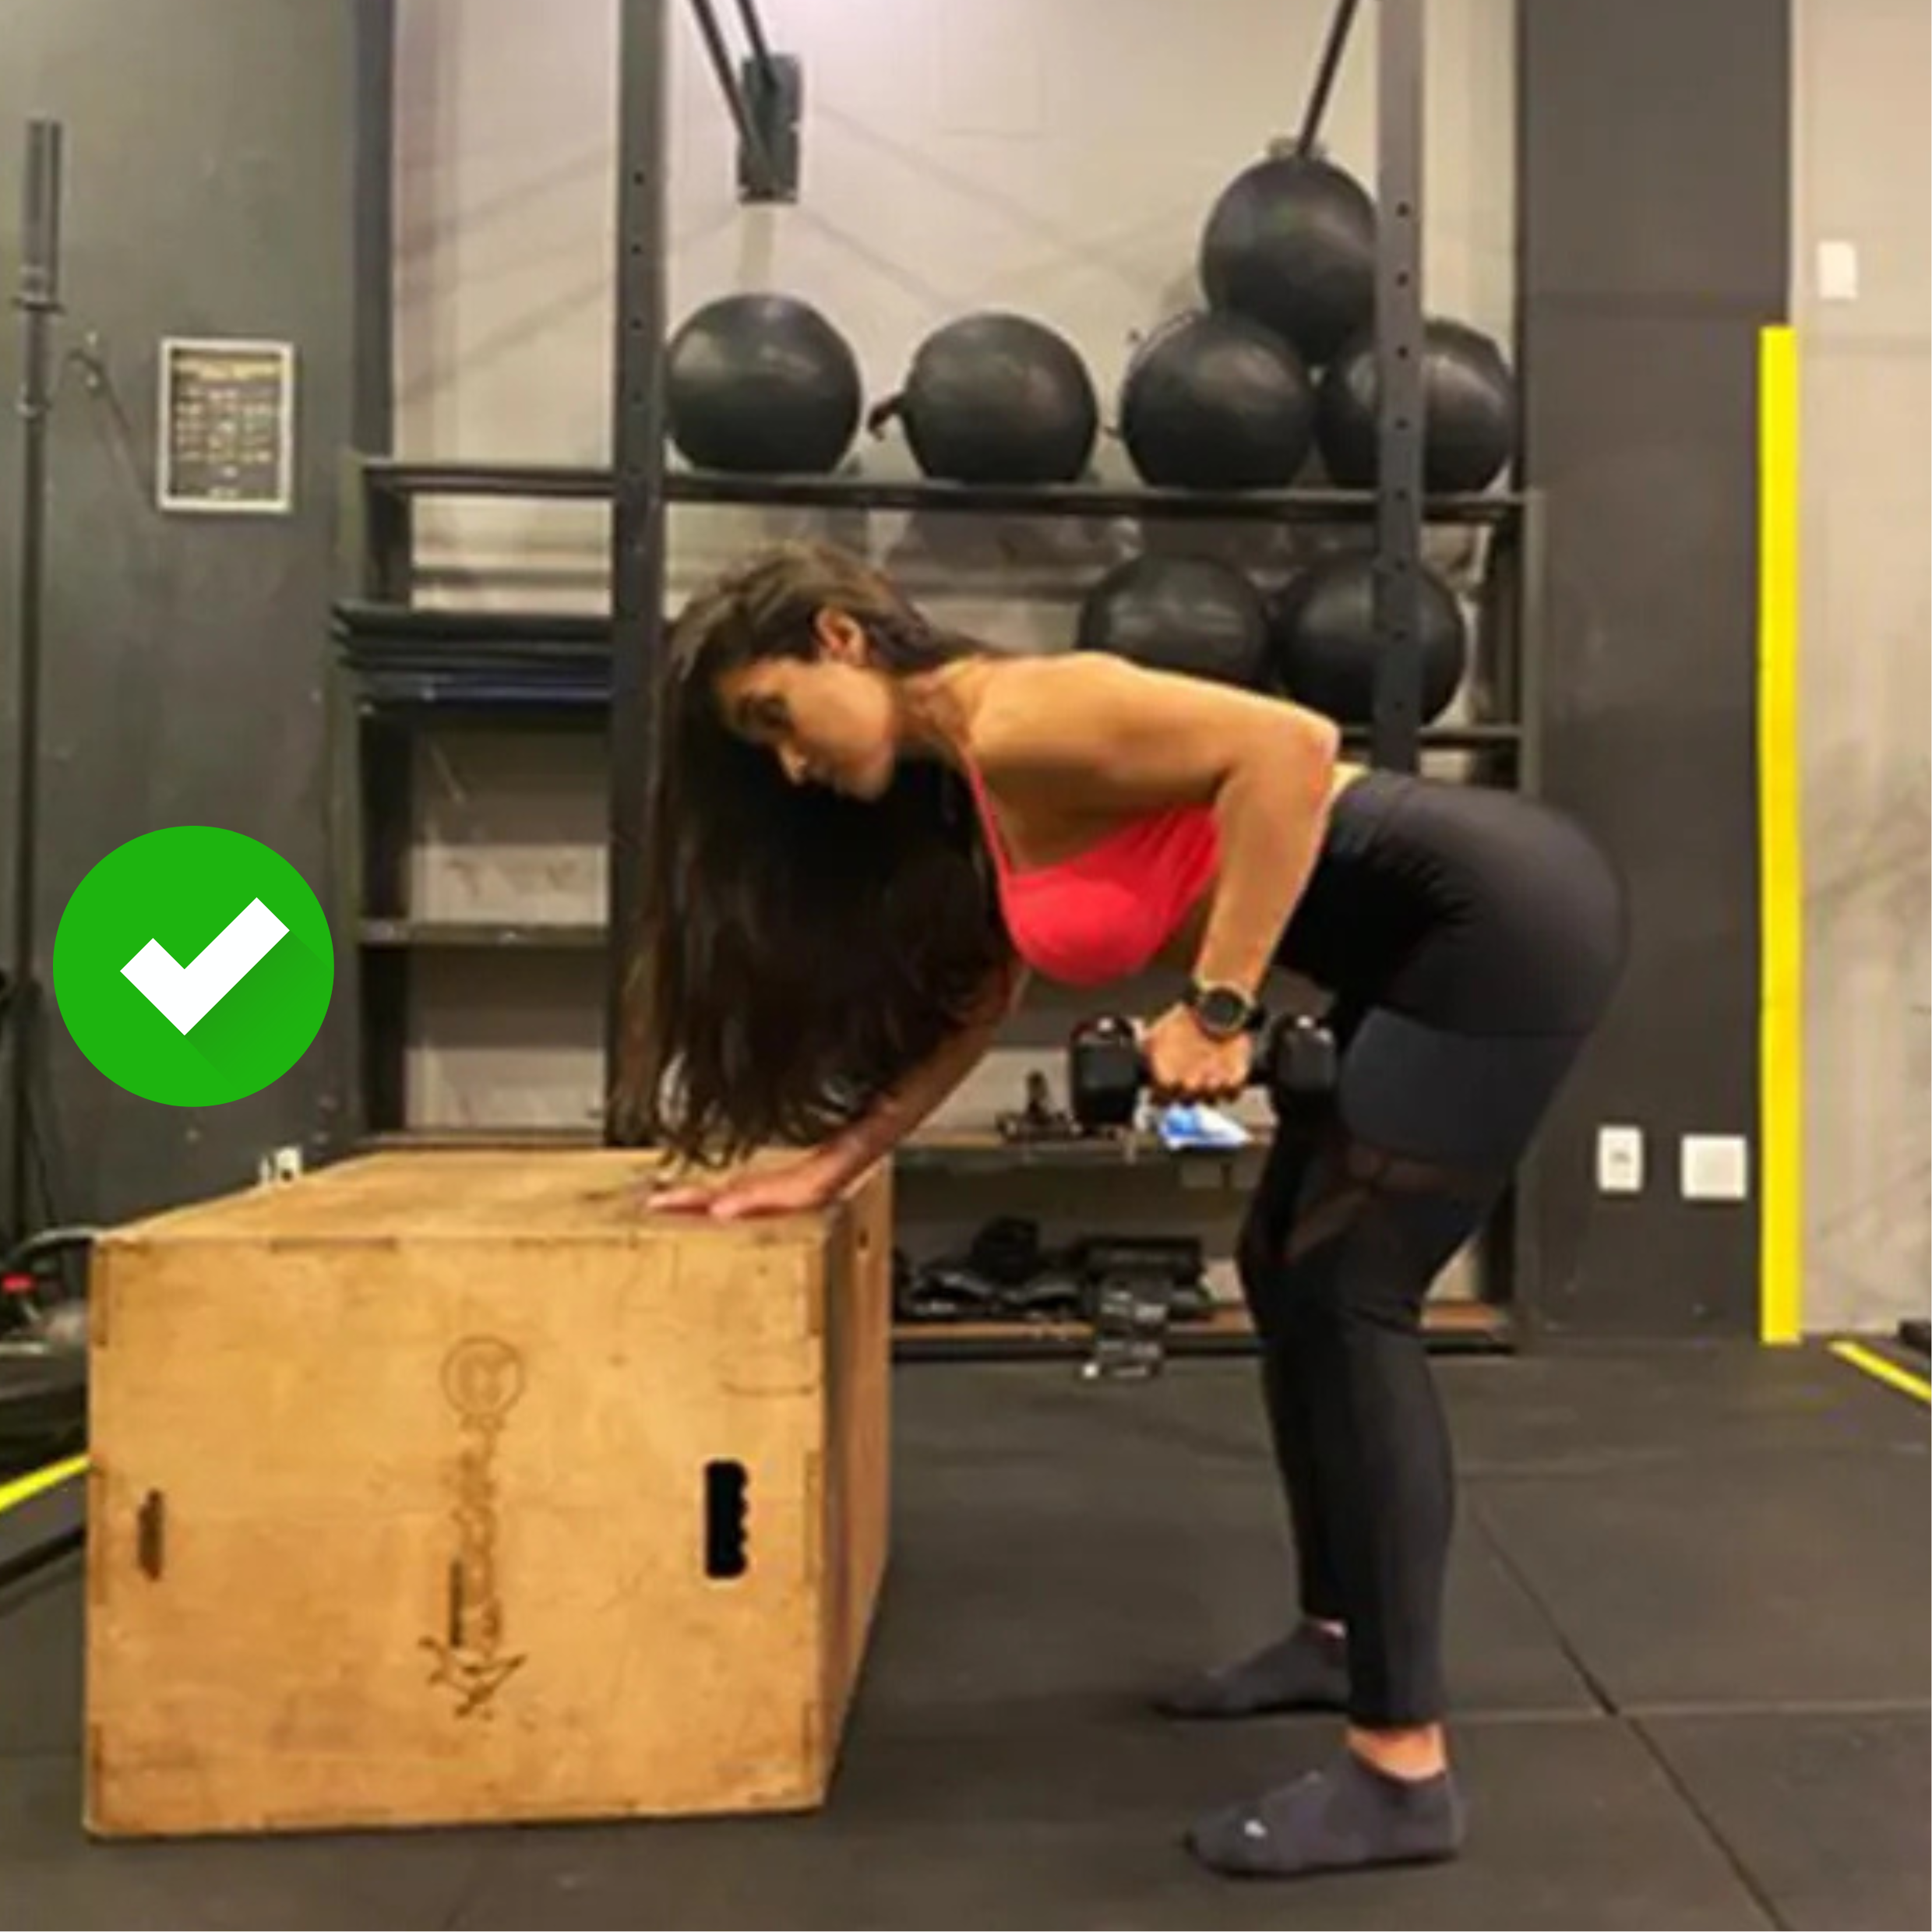
\includegraphics[width=0.45\textwidth]{imgs/imagens/3.png}
        \label{fig:remada_correto}
    }
    \hfill
    \subfigure[Execução incorreta]{%
        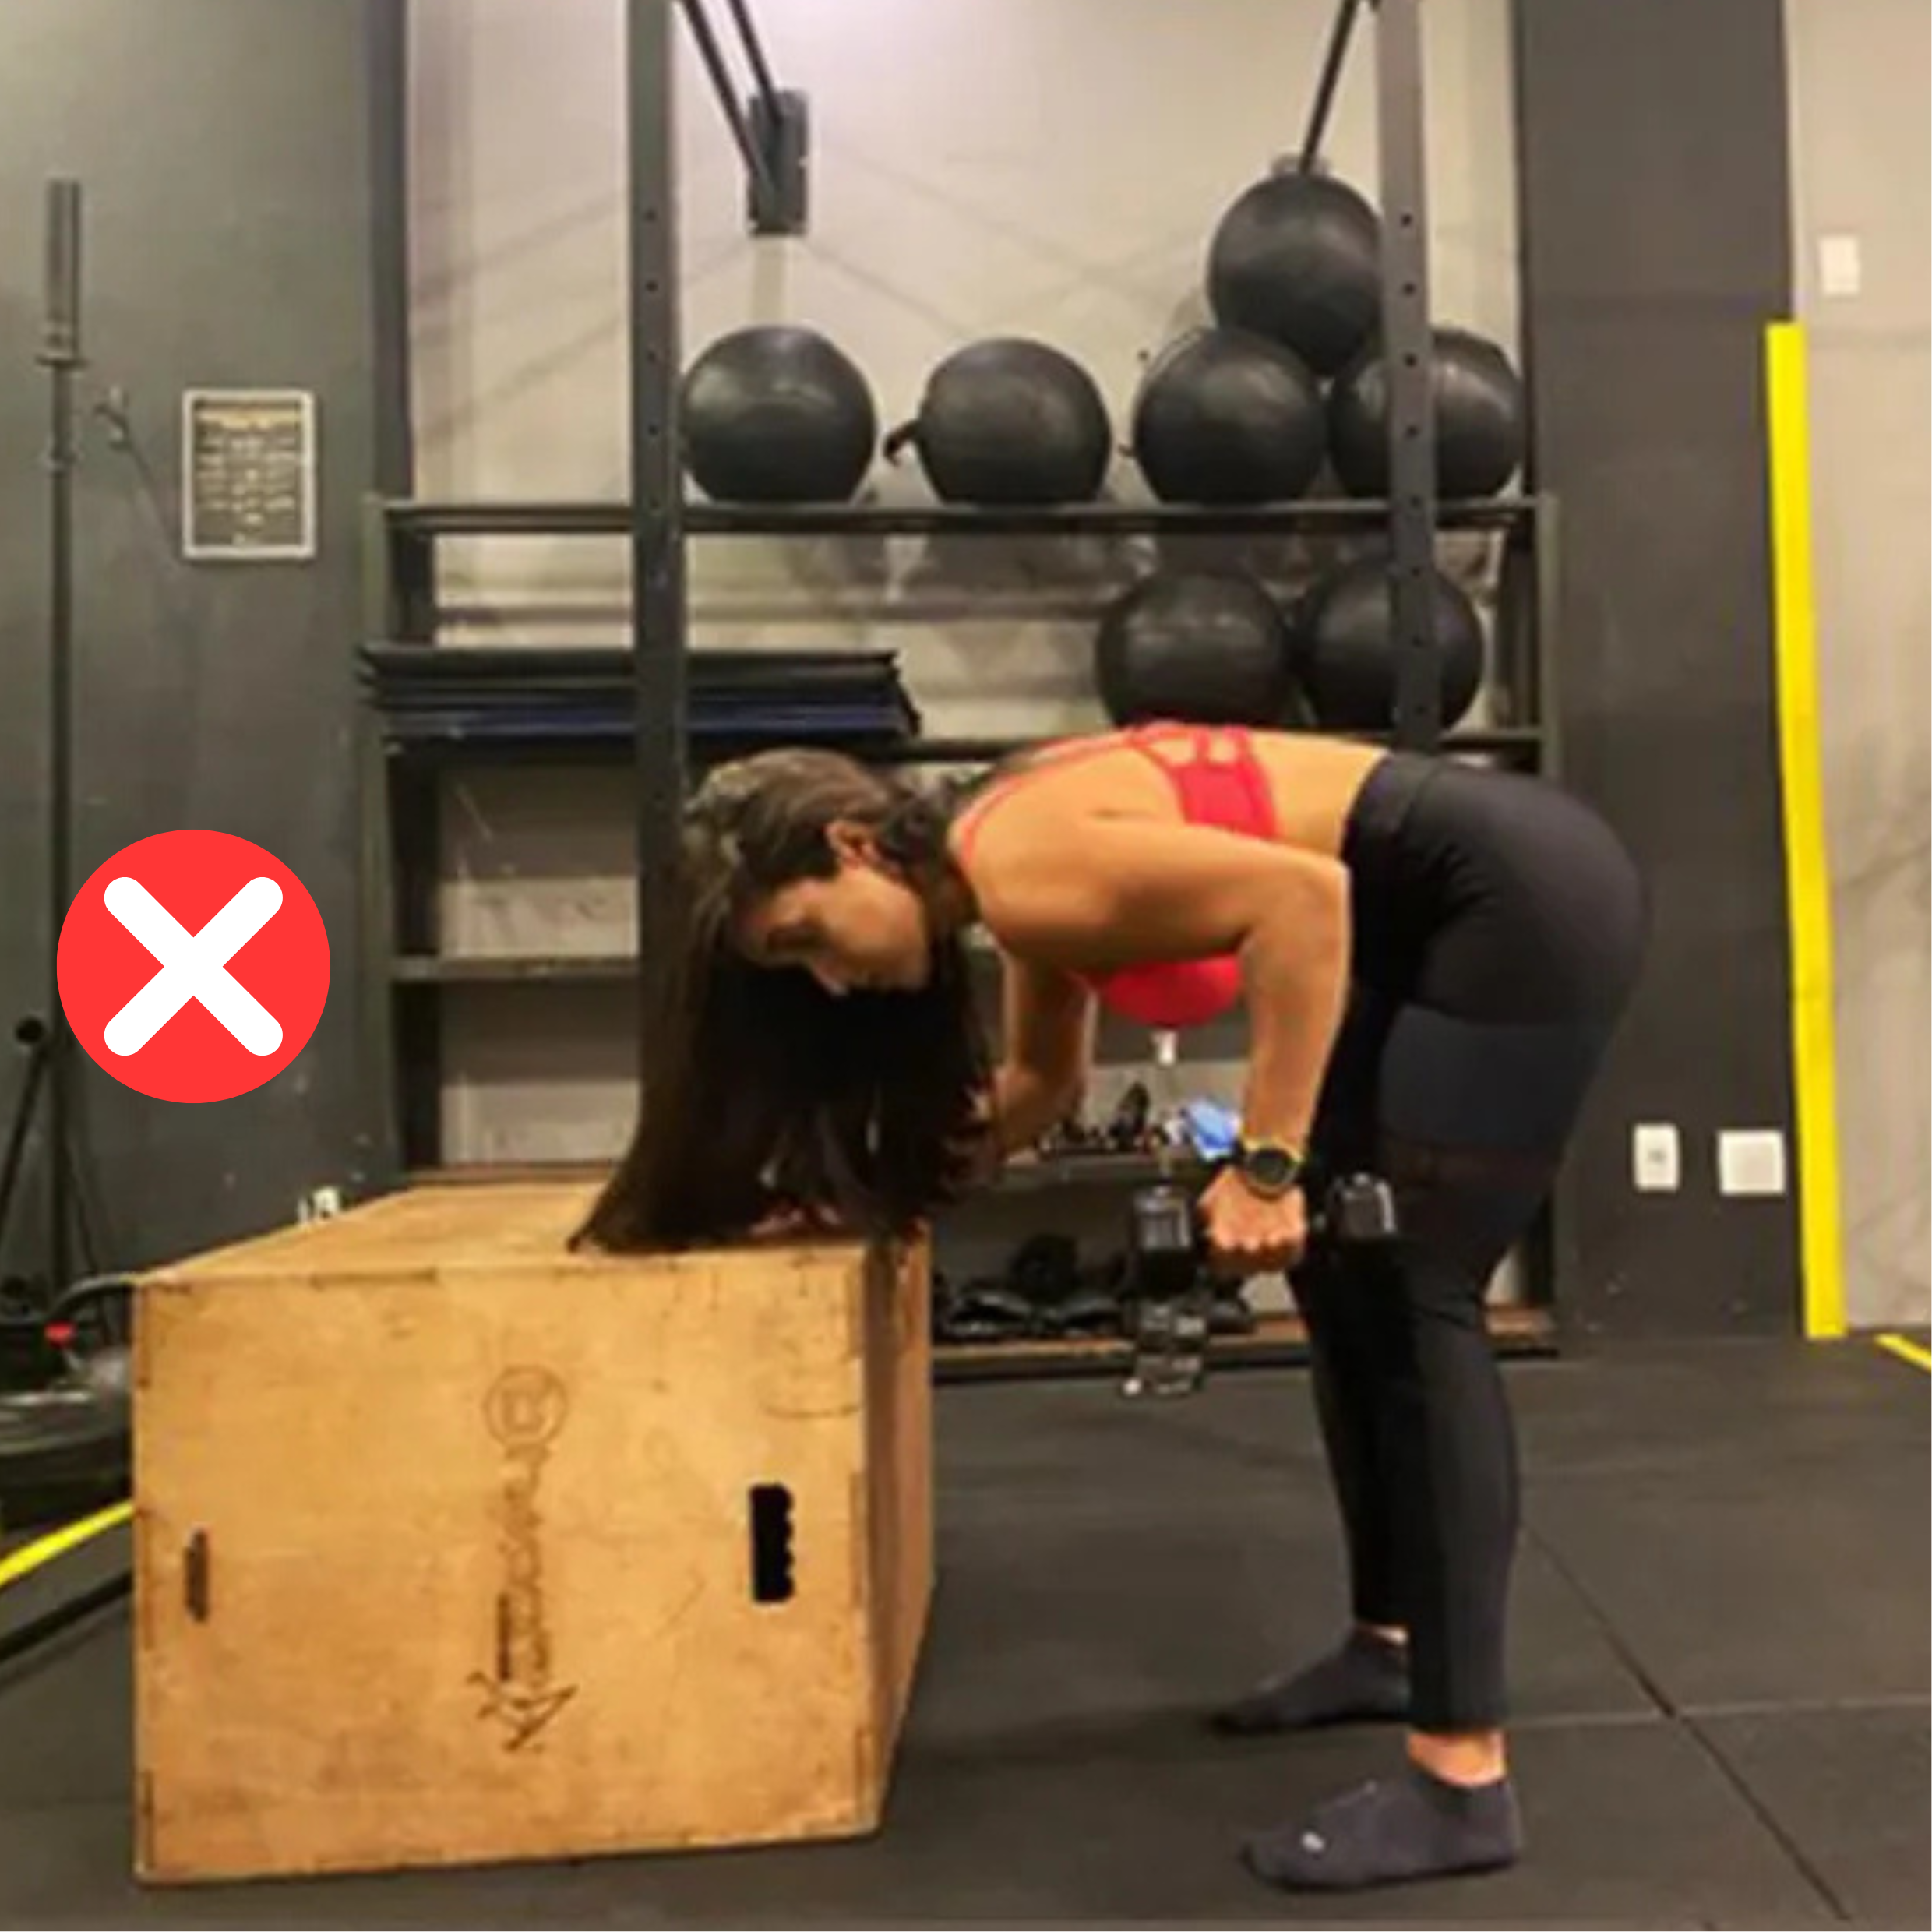
\includegraphics[width=0.45\textwidth]{imgs/imagens/4.png}
        \label{fig:remada_incorreto}
        }
    \fonte{\citeonline{globo2023-exercicios} adaptado pelo Autor.}
\end{figure}

\begin{figure}[H]
    \centering
    \caption{Exemplo de execução correta (a) e incorreta (b) do exercício de desenvolvimento de ombro. }
    \subfigure[Execução correta]{%
        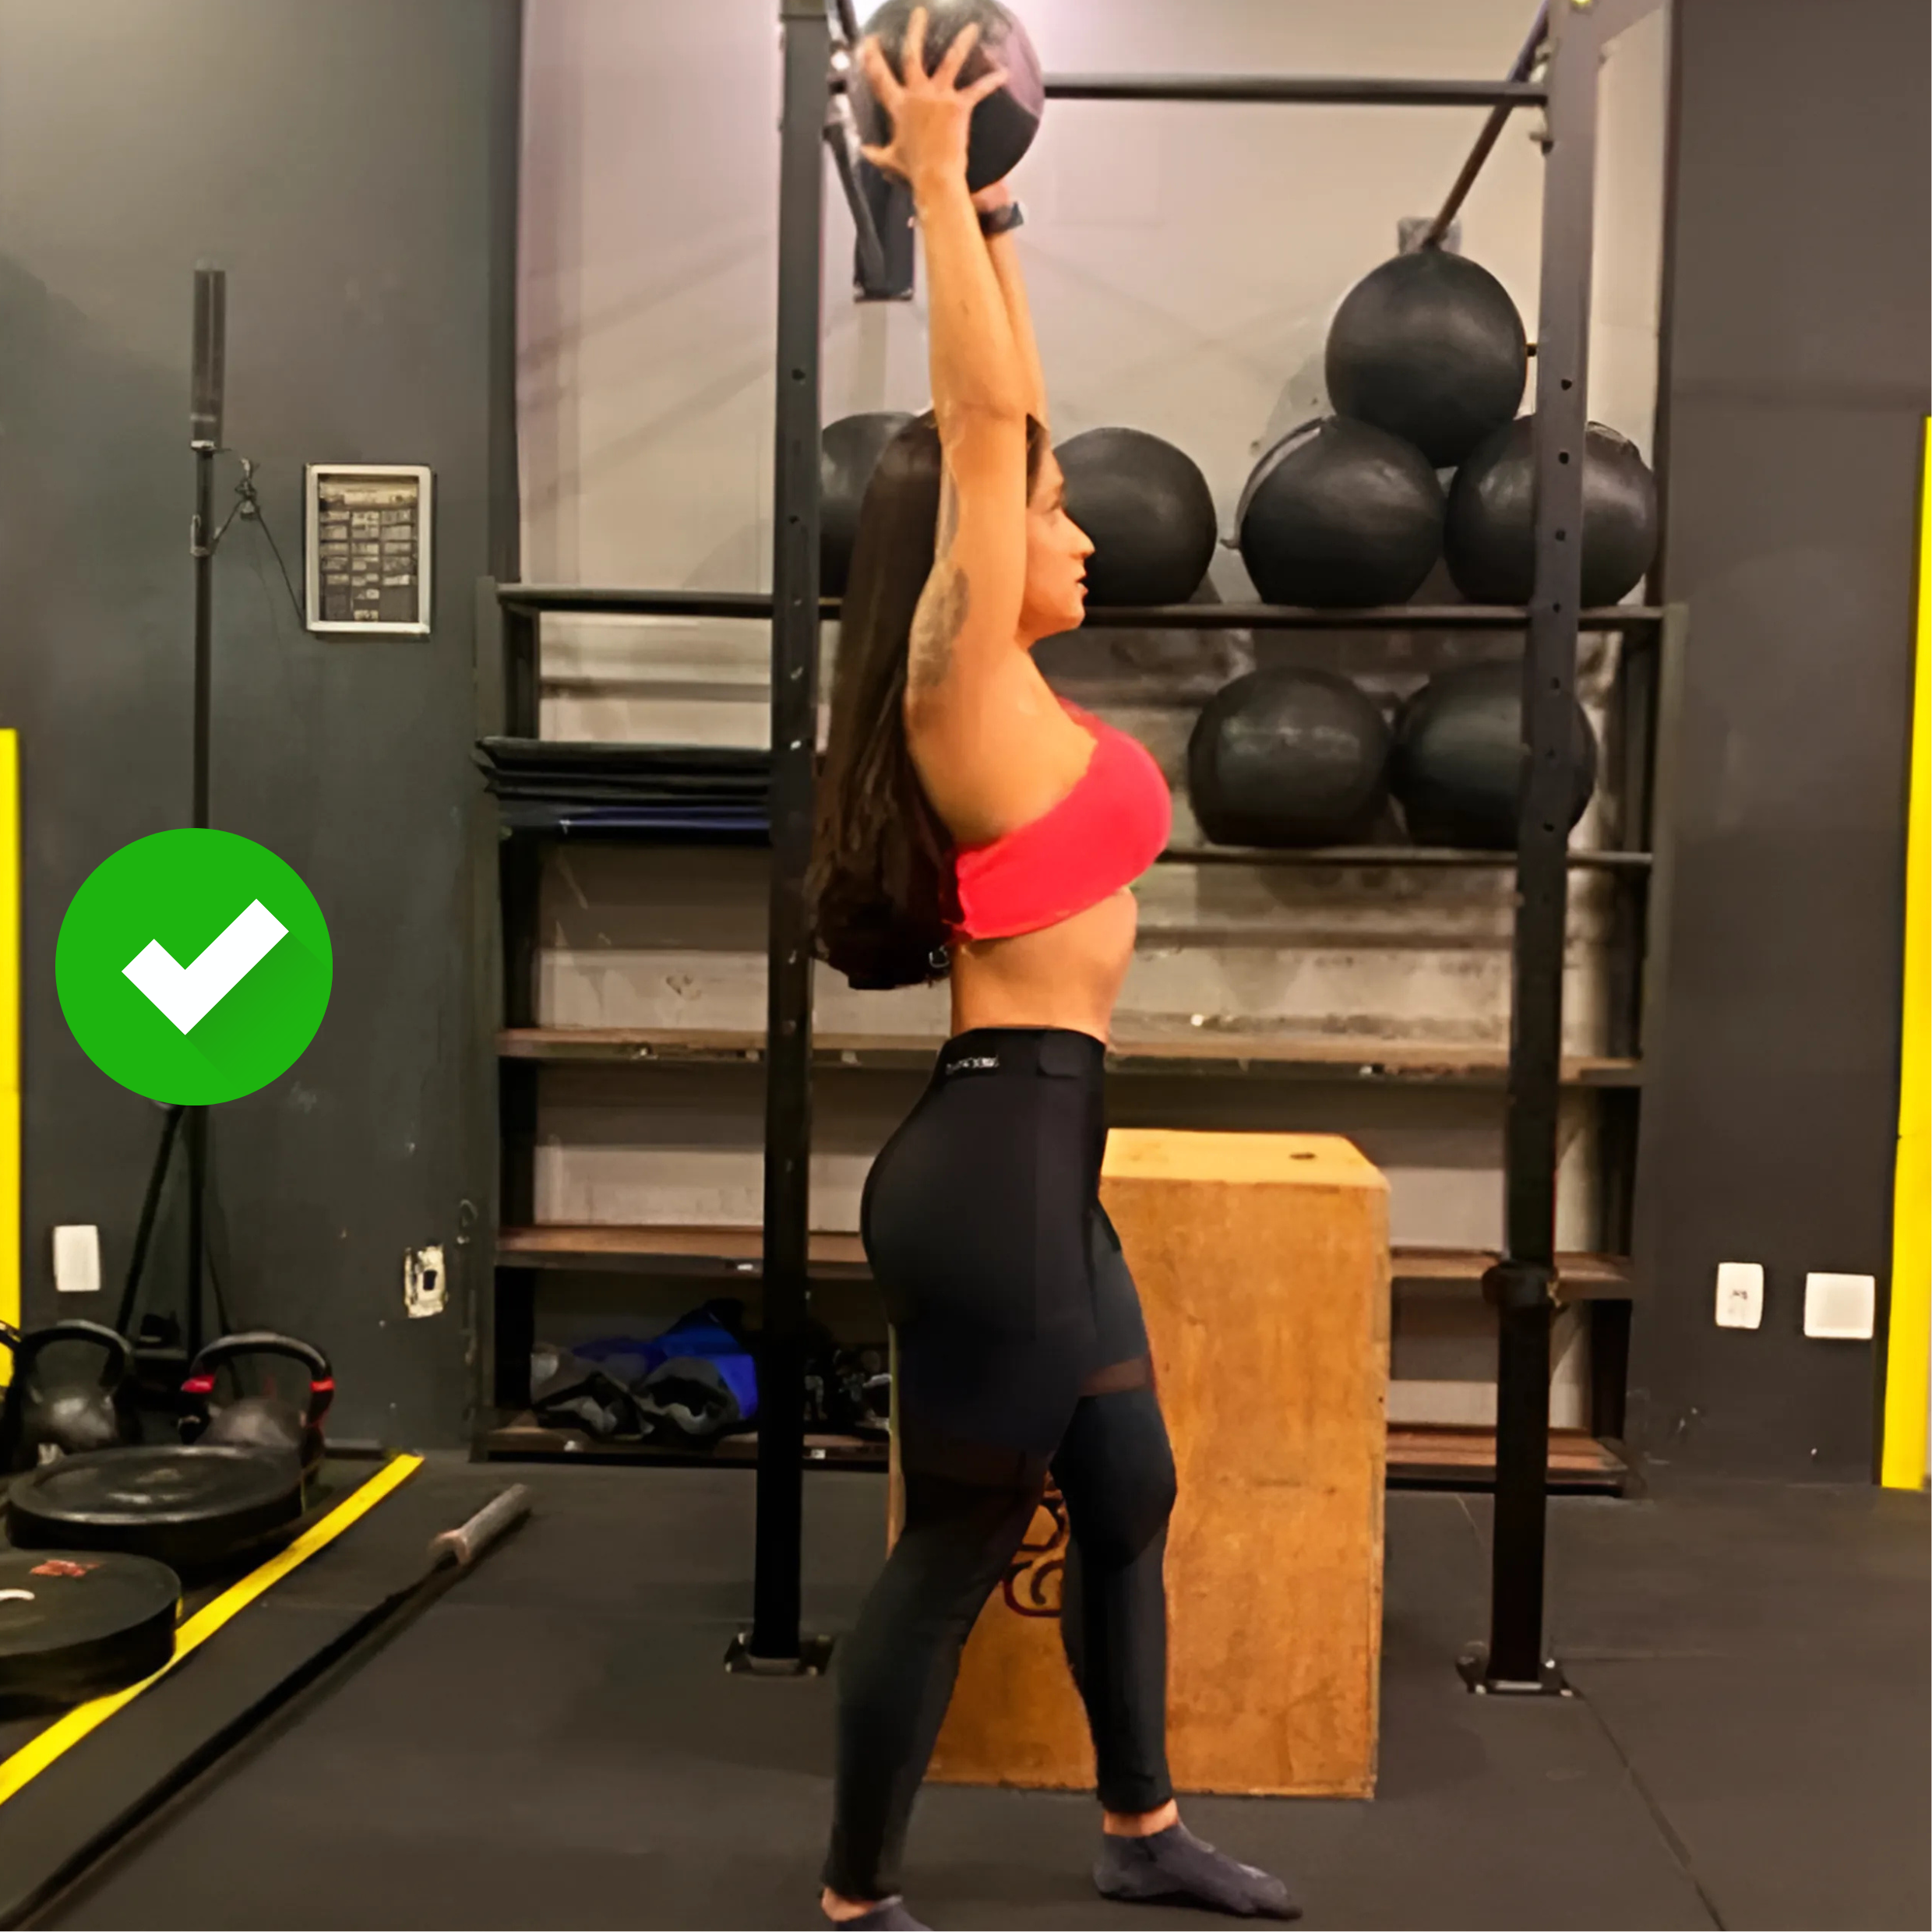
\includegraphics[width=0.45\textwidth]{imgs/imagens/2.png}
        \label{fig:desenvolvimento_correto}
    }
    \hfill
    \subfigure[Execução incorreta]{%
        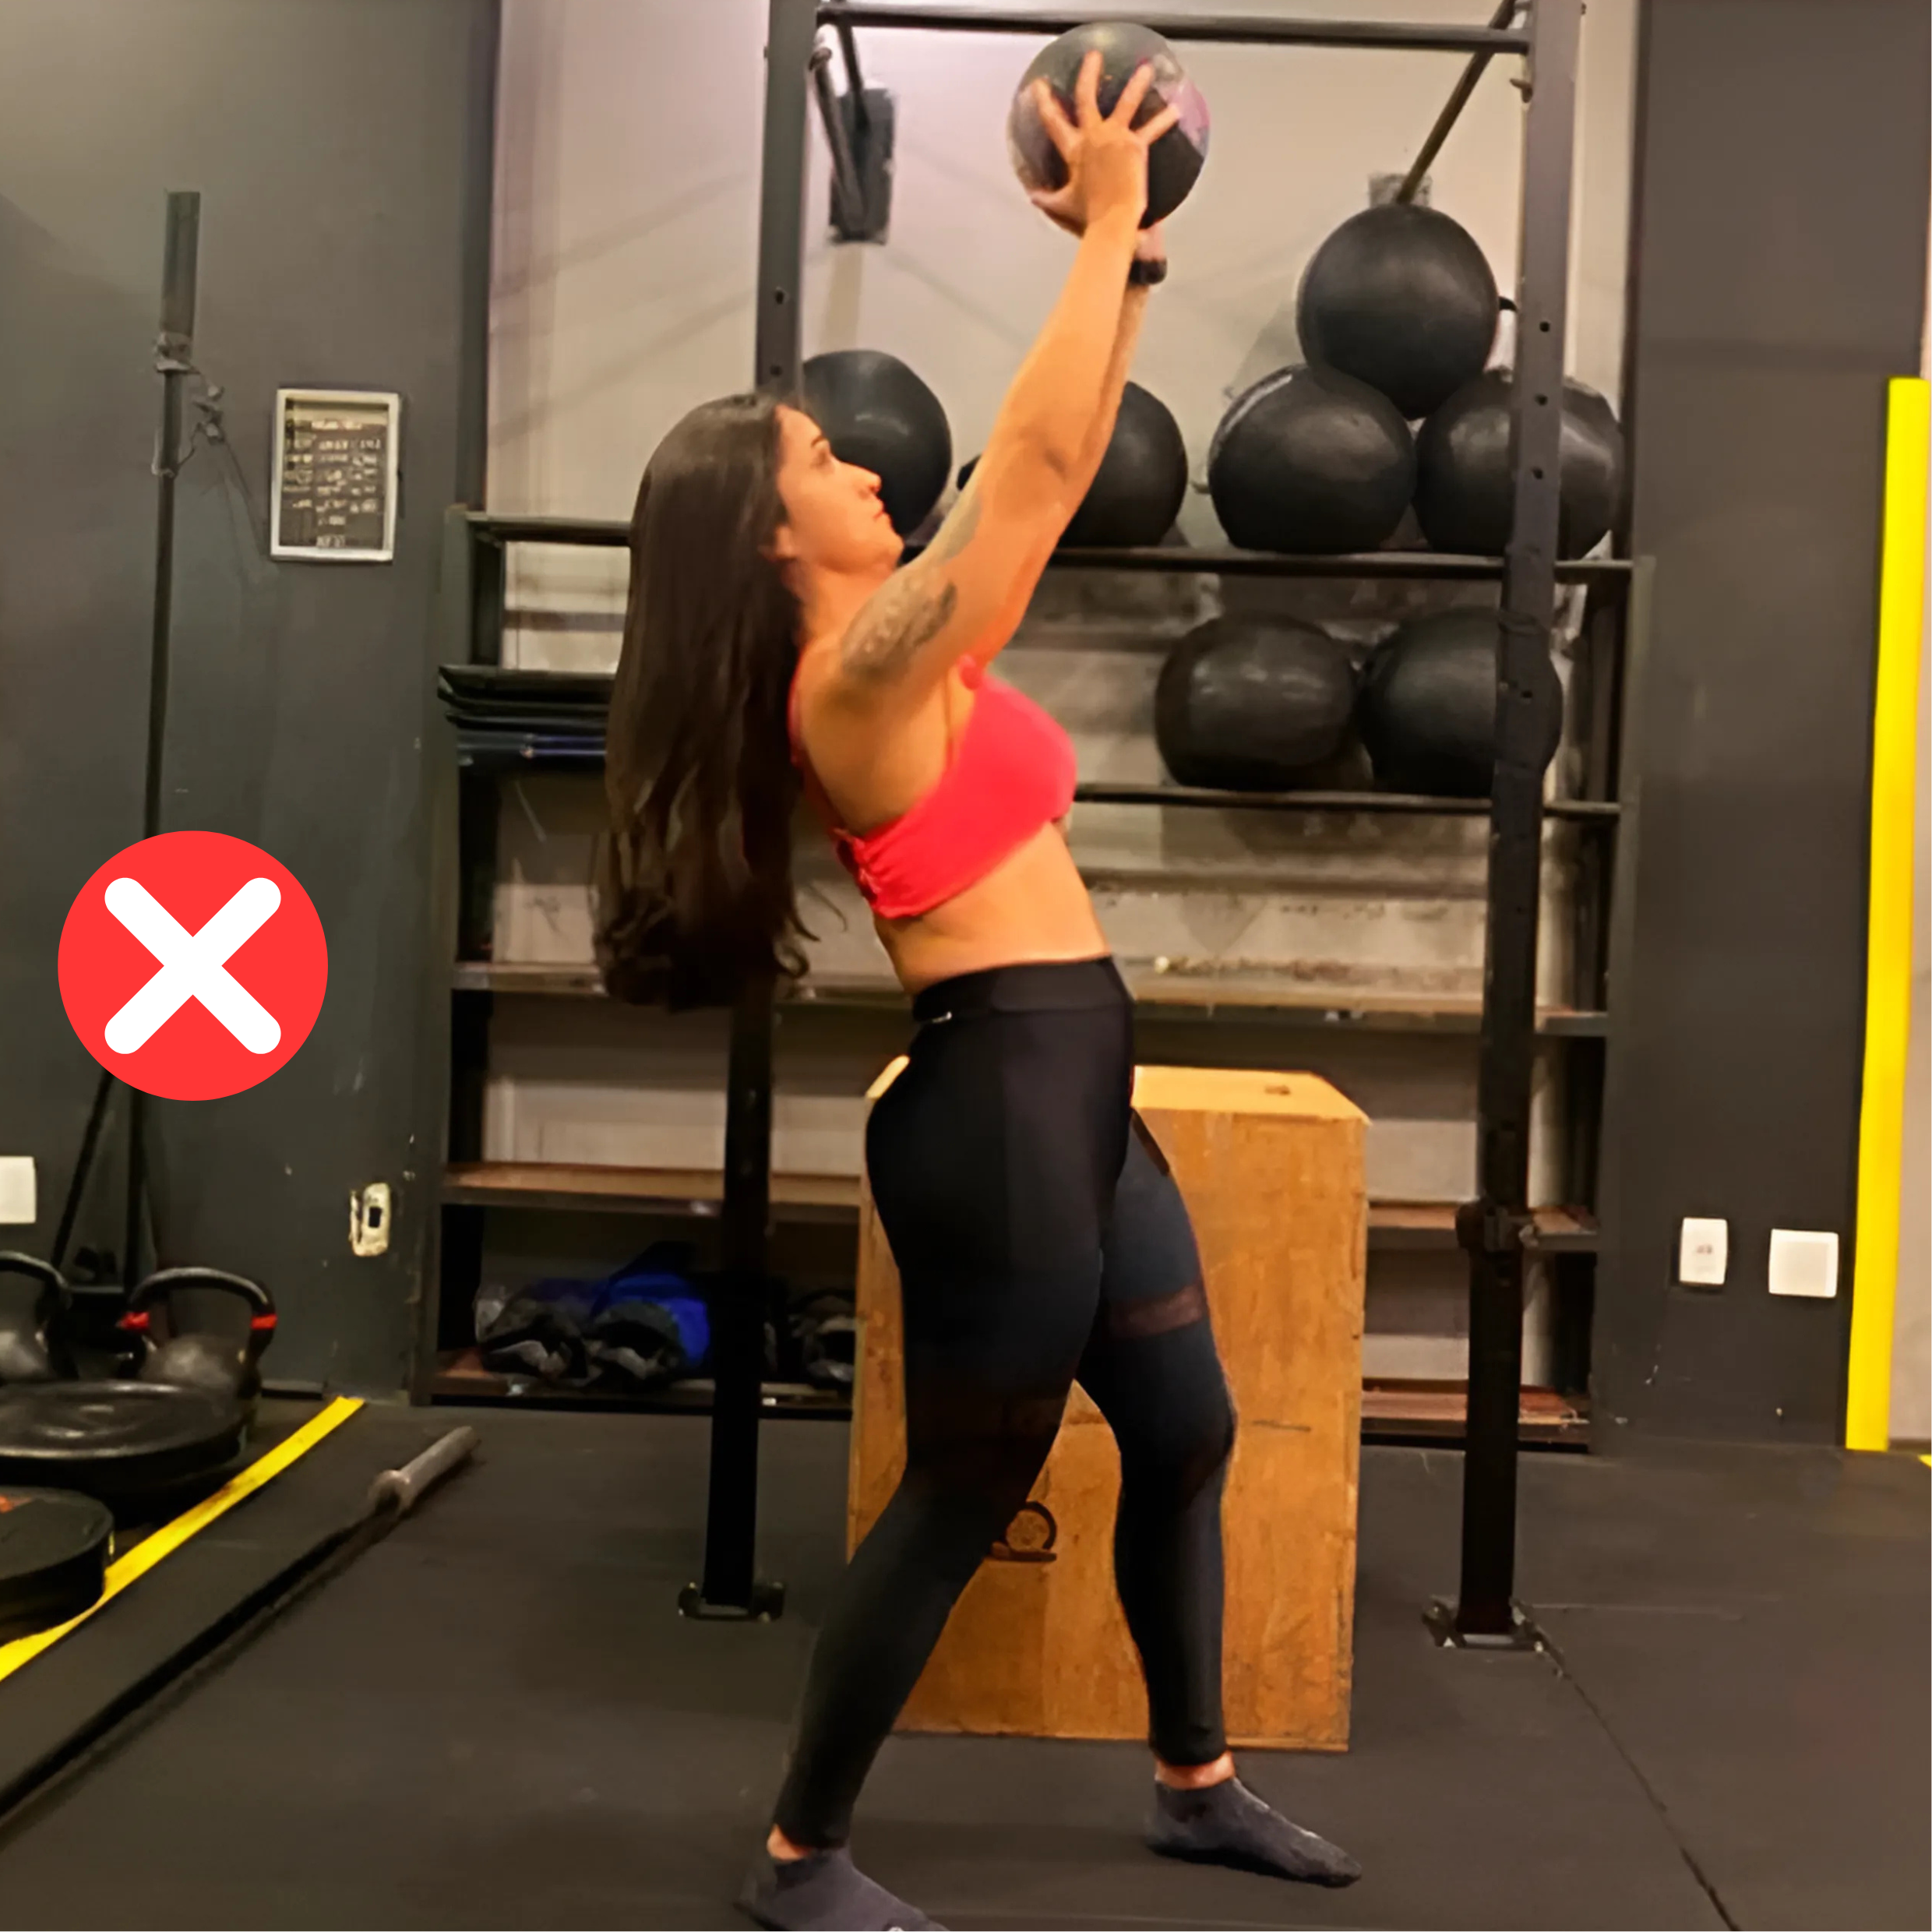
\includegraphics[width=0.45\textwidth]{imgs/imagens/1.png}
        \label{fig:desenvolvimento_incorreto}
    }
    \fonte{\citeonline{globo2023-exercicios} adaptado pelo Autor.}
\end{figure}

As máquinas, por sua vez, oferecem maior segurança e estabilidade, já que guiam o movimento e reduzem a necessidade de estabilização. Isso as torna indicadas para iniciantes, reabilitação e treinos específicos. Entretanto, apresentam custo elevado, menor portabilidade e menor ativação de músculos estabilizadores em comparação aos pesos livres. Exercícios com elásticos ou peso corporal também podem ser empregados, especialmente em contextos de treinamento funcional, em programas de baixo custo ou em situações de reabilitação \cite{murer-treinamento-2022}.

A biomecânica exerce o papel de análise do treinamento de força, pois permite compreender as forças internas (produzidas pelos músculos e transmitidas pelas articulações) e externas (como a gravidade e a resistência imposta por equipamentos) atuantes durante o movimento. Essa análise envolve variáveis como amplitude de movimento, torque articular, planos de execução, vetores de força e tipos de ação muscular (concêntrica, excêntrica e isométrica) \cite{emmanouil-two-2024,murer-treinamento-2022}. A relação entre essas variáveis influencia diretamente as adaptações fisiológicas e o risco de lesão.  

Erros de execução — como desalinhamento postural, amplitude incorreta ou cadência inadequada — estão associados a distensões, tendinopatias e sobrecargas articulares. Movimentos multiarticulares, como o agachamento e o levantamento terra, são especialmente críticos por envolverem grandes grupos musculares e elevadas cargas compressivas sobre a coluna lombar \cite{william-j-kraemer-fundamentos-2021,chen-analysis-2024}.  

Nesse cenário, torna-se cada vez mais importante a presença de feedback em tempo real, capaz de auxiliar na postura, identificar padrões inadequados e corrigir erros antes que comprometam a segurança ou a eficácia do exercício \cite{dzaja-quantitative-nodate,chen-analysis-2024,balkhi-multipurpose-nodate}.

\section{Sensores Inerciais (IMUs)}

As Unidades de Medição Inercial (IMUs, do inglês \textit{Inertial Measurement Units}) são dispositivos capazes de medir grandezas físicas associadas ao movimento, como aceleração linear, velocidade angular e, em alguns casos, orientação magnética. Geralmente integram três sensores principais: acelerômetro, giroscópio e magnetômetro, permitindo medições em até seis graus de liberdade \cite{BMI160,ICM20602}.  

Graças ao seu baixo custo, reduzido consumo de energia e portabilidade, as IMUs tornaram-se amplamente utilizadas em smartphones, dispositivos vestíveis, veículos autônomos, realidade aumentada, robótica e em diferentes aplicações biomédicas e esportivas \cite{BMI160,ICM42688P}. Cada sensor possui características próprias. O acelerômetro mede a aceleração linear em três eixos, sendo sensível tanto à gravidade quanto a movimentos dinâmicos. O giroscópio fornece informações sobre a velocidade angular, permitindo detectar rotações, mas sofre com o problema da deriva (\textit{drift}) ao longo do tempo. Já o magnetômetro mede o campo magnético local e pode auxiliar na estimativa da orientação, embora seja sensível a interferências ambientais \cite{ADXL335}. Os modelos mais comuns, como o MPU-60X0, o BMI160 e a família ICM (ICM-20602, ICM-42688-P), combinam acelerômetros e giroscópios em um único chip de silício, permitindo medições de seis graus de liberdade (6-DoF), as Figuras \ref{fig:imu_acc} e \ref{fig:imu_gyro} mostram um exemplo de um chipe MPU-6050, que integra um acelerômetro e um giroscópio.

\begin{figure}[H]
    \centering
    \caption{Exemplo de chipe Acelerômetro e Giroscópio MPU-6050.}
    \subfigure[Medir aceleração]{%
        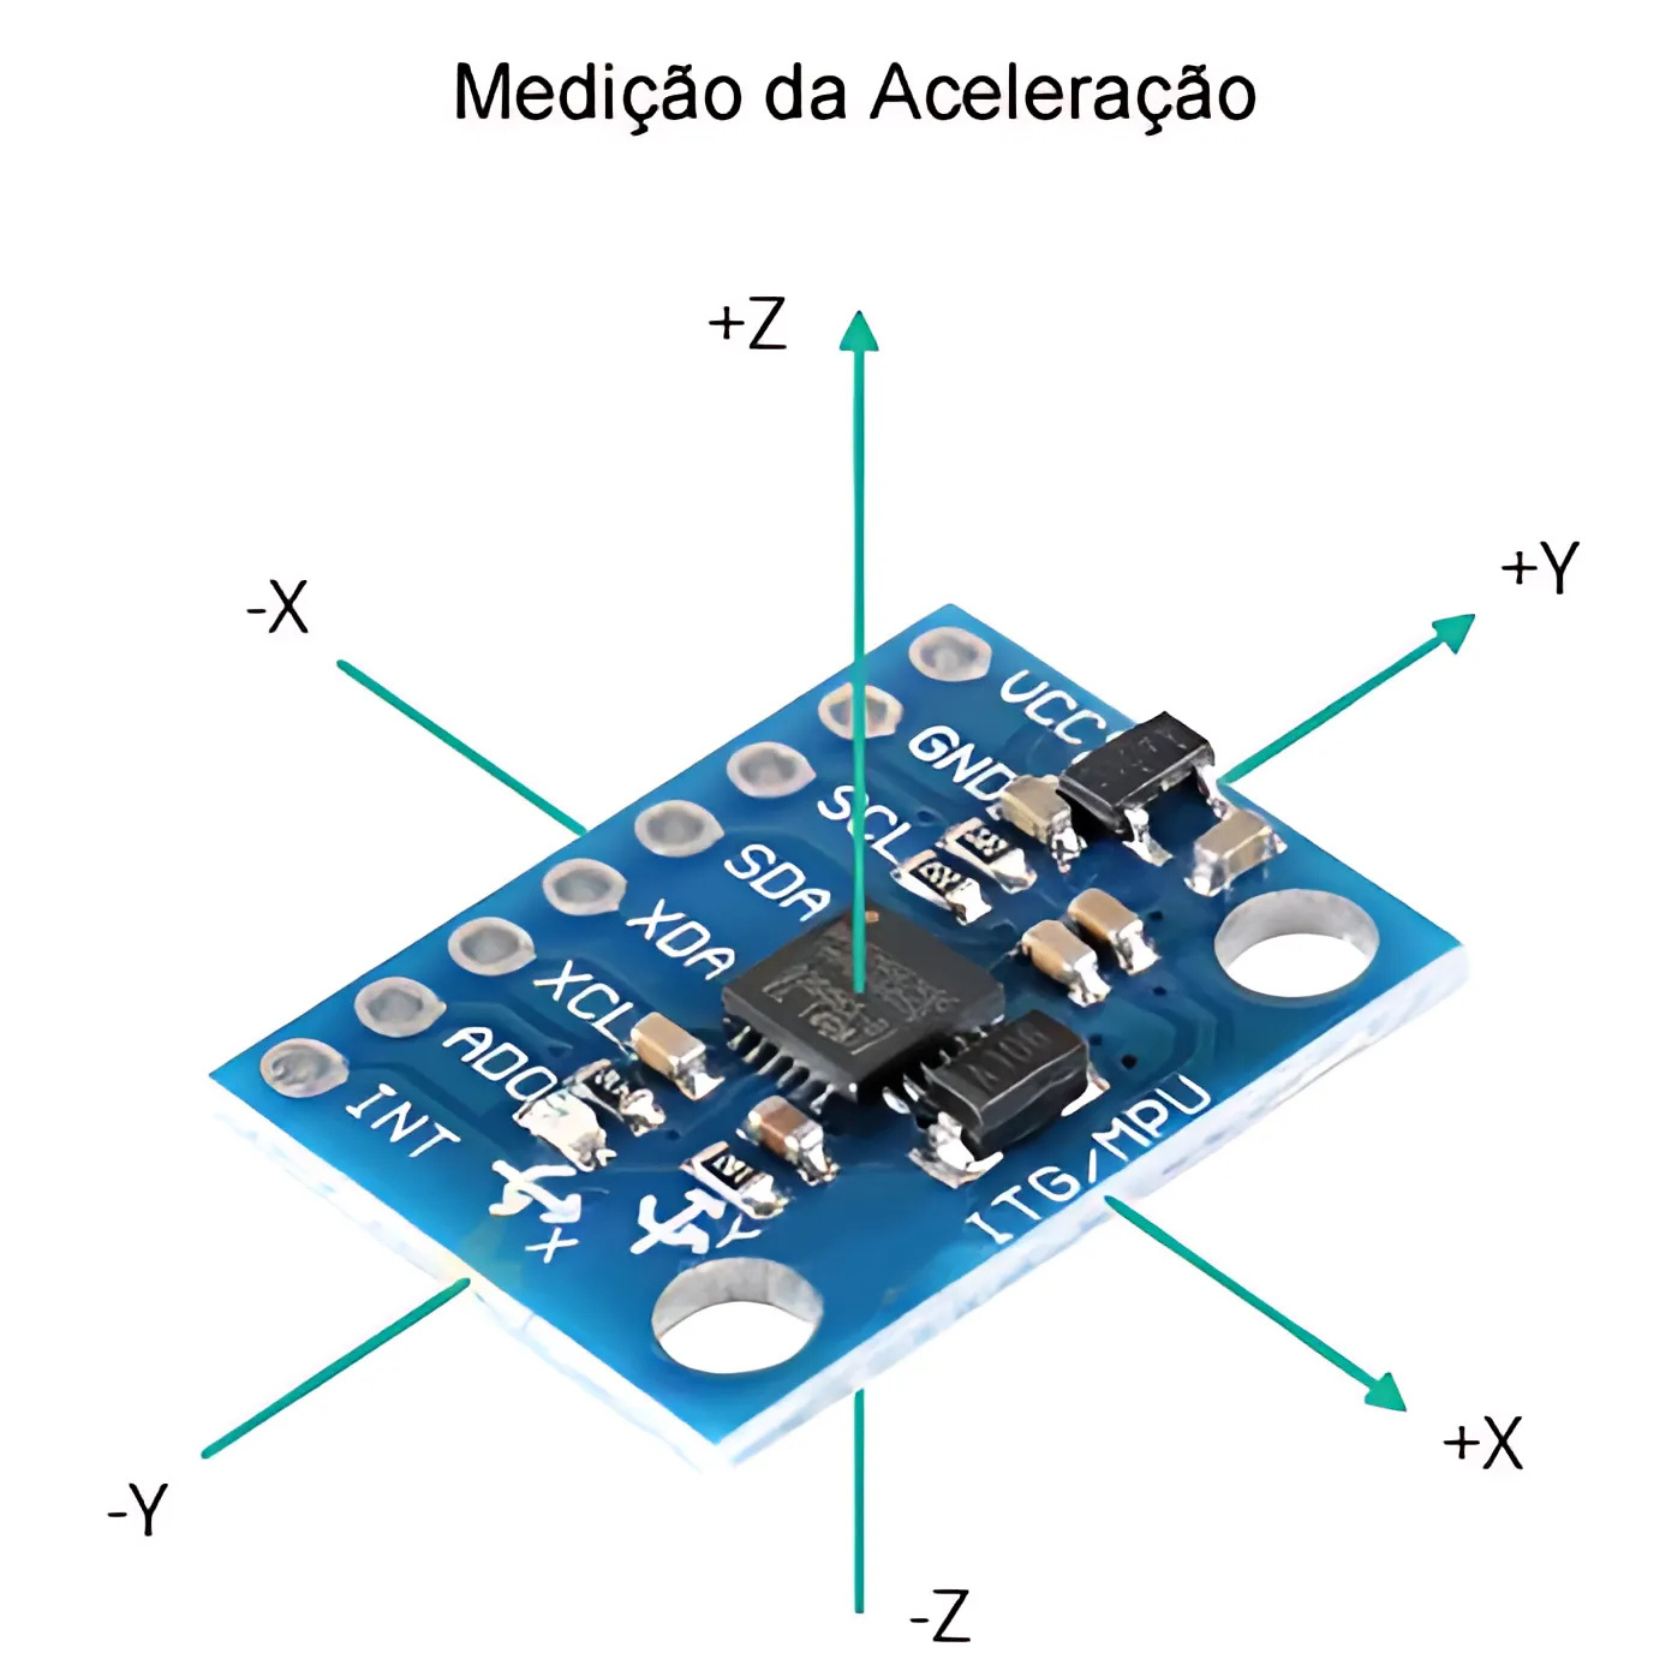
\includegraphics[width=0.45\textwidth]{imgs/imagens/6.png}
        \label{fig:imu_acc}
    }
    \hfill
    \subfigure[Medir rotação]{%
        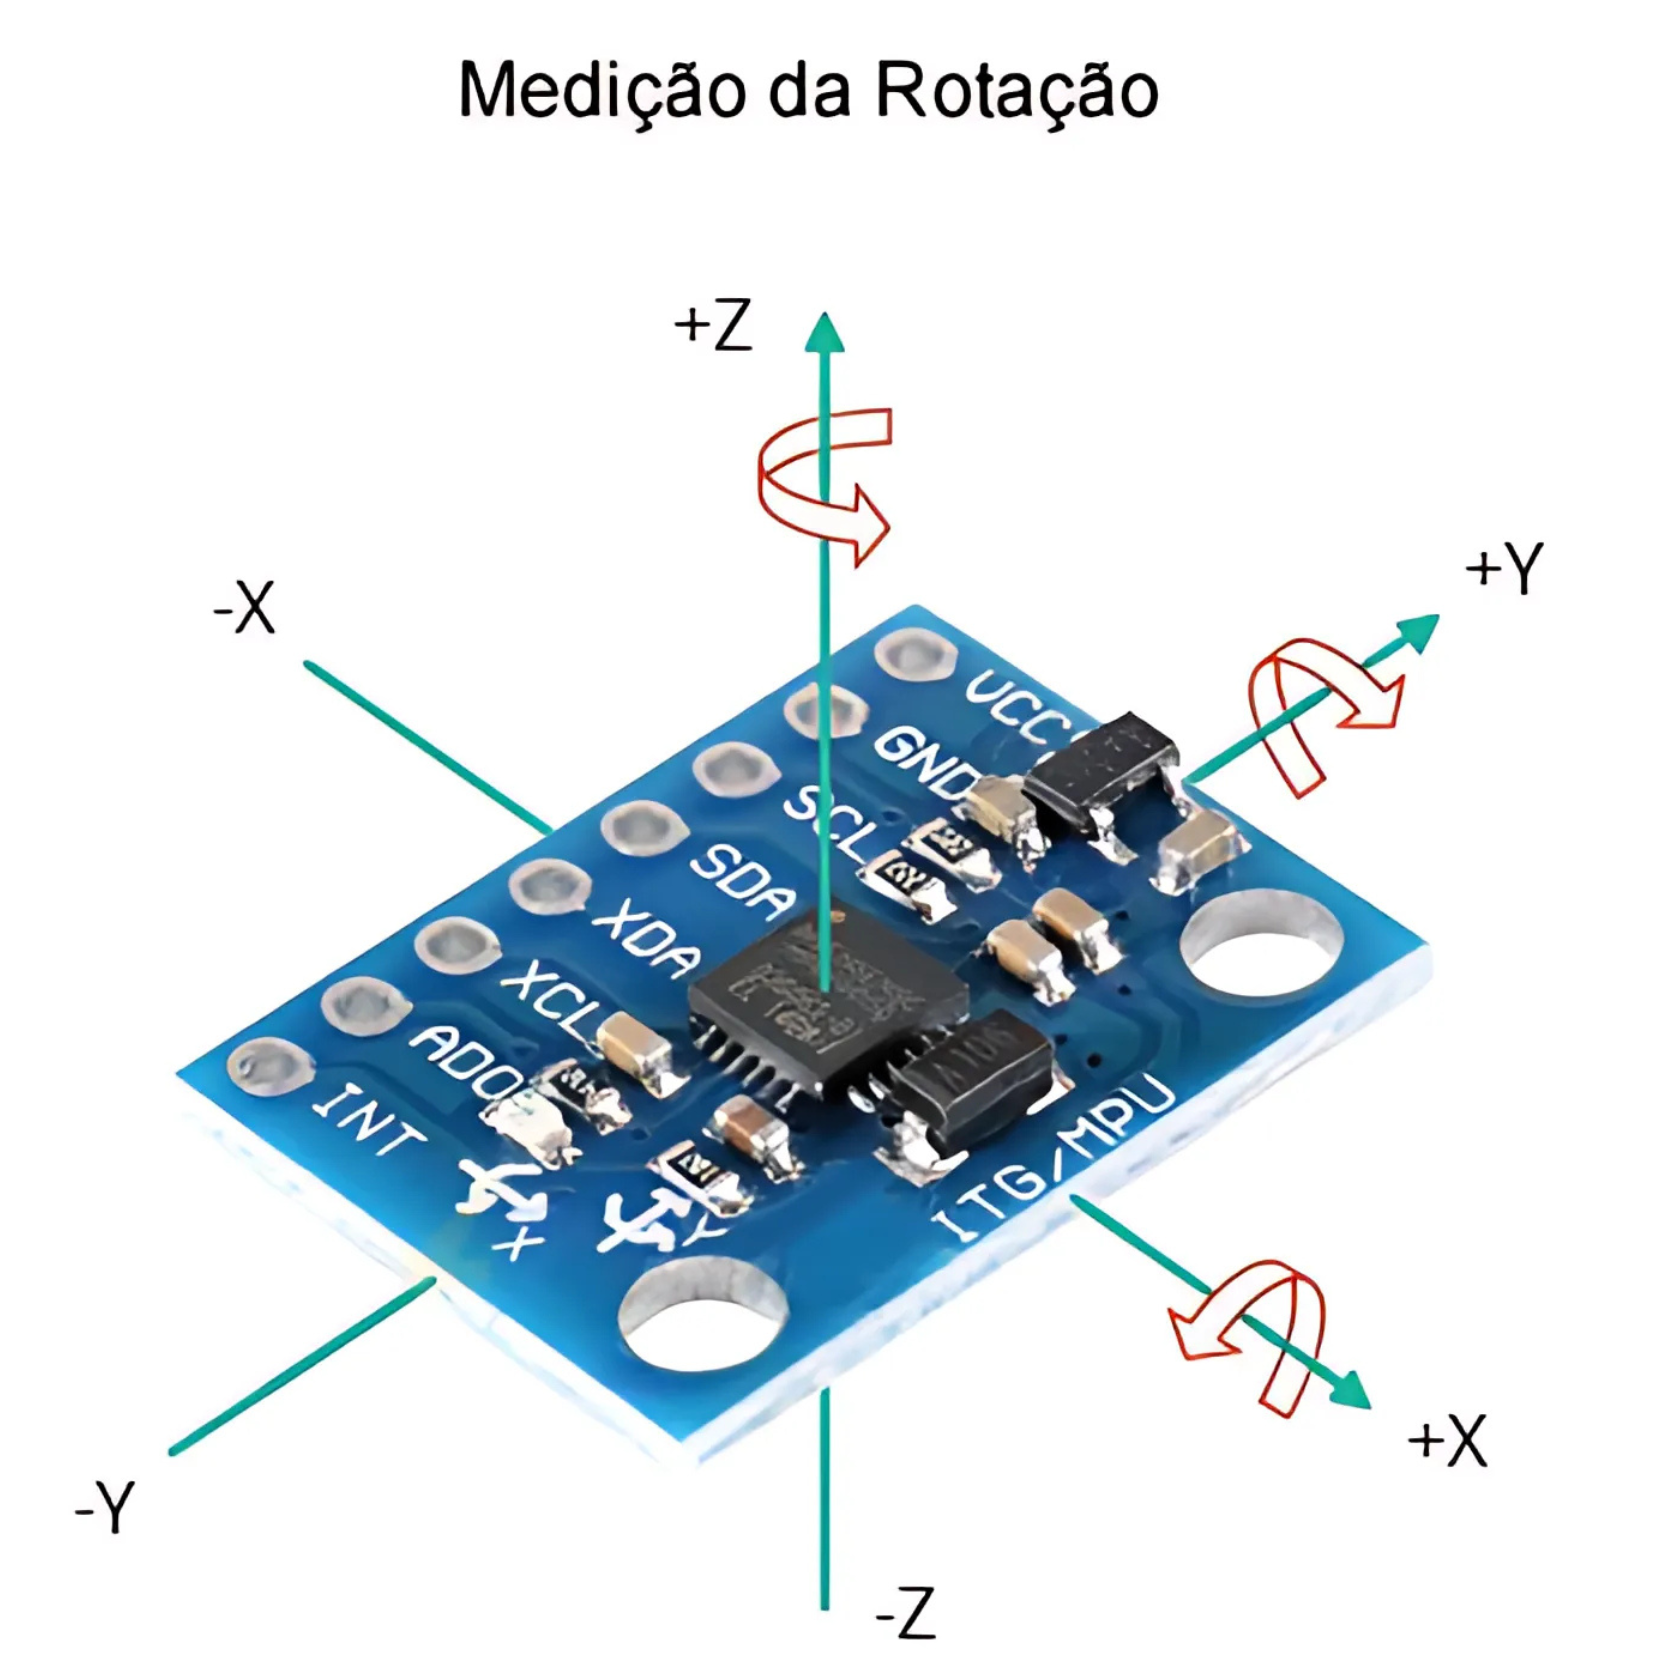
\includegraphics[width=0.45\textwidth]{imgs/imagens/7.png}
        \label{fig:imu_gyro}
        }
    \fonte{\citeonline{usinainfo-mpu6050} adaptado pelo Autor.}
\end{figure}

Para aumentar a confiabilidade das medições, técnicas de fusão sensorial (\textit{sensor fusion}) combinam os sinais dos diferentes sensores, compensando as limitações individuais. Filtros como o de Kalman e o de Madgwick são amplamente empregados para reduzir ruídos e melhorar a precisão na estimativa da orientação e da postura corporal \cite{BMI160}.  

No campo da análise de movimento humano, as IMUs permitem monitorar a inclinação, a amplitude de movimento, a postura e a execução de gestos motores. Isso viabiliza tanto o monitoramento contínuo de atividades quanto o fornecimento de feedback em tempo real. Contudo, seu uso ainda apresenta desafios importantes. Problemas como ruídos e deriva podem comprometer a acurácia da estimativa de posição ao longo do tempo, enquanto falhas de calibração ou erros no posicionamento do sensor em relação ao corpo resultam em medições imprecisas. A autonomia de bateria também é uma limitação, especialmente em aplicações contínuas. Além disso, diferenças individuais, como anatomia, técnica e nível de experiência, impactam a generalização de modelos de reconhecimento treinados em bases de dados restritas, exigindo estratégias específicas para adaptação a cada usuário \cite{dzaja-quantitative-nodate,balkhi-multipurpose-nodate}.  

Apesar dessas dificuldades, pesquisas recentes demonstram que uma única IMU, bem posicionada, pode identificar diferentes exercícios com acurácia superior a 90\% \cite{balkhi-multipurpose-nodate,pinto-aplicacao-2023}. A integração desses sensores diretamente em equipamentos, como halteres, surge como alternativa para elimina a necessidade de múltiplos sensores corporais e reduz o desconforto do usuário, ao mesmo tempo em que possibilita coleta de dados rica e precisa para avaliação da qualidade do movimento.

\section{Monitoramento de Exercícios com Sensores}

O monitoramento automatizado de exercícios tem ganhado destaque nos últimos anos, impulsionado tanto pela popularização do treinamento com pesos quanto pela necessidade de programas individualizados que garantam maior segurança e eficiência \cite{pinto-aplicacao-2023}. A incorporação de tecnologias nesse processo busca reduzir o risco de lesões, melhorar a técnica de execução e aumentar a motivação dos praticantes, suprindo limitações do acompanhamento humano, que depende de observação direta, disponibilidade de profissionais e pode ser influenciado pela subjetividade \cite{dzaja-quantitative-nodate,balkhi-multipurpose-nodate,gupta-yogahelp-2021}.  

Diferentes abordagens tecnológicas vêm sendo exploradas. Os sistemas baseados em visão computacional alcançam níveis elevados de precisão na análise da postura e na identificação de movimentos, mas apresentam desvantagens como alto custo, dependência de infraestrutura adequada e questões de privacidade. Já os dispositivos vestíveis, em especial os que utilizam IMUs, destacam-se por serem mais acessíveis, portáteis e capazes de funcionar em ambientes variados. Esses sensores permitem identificar exercícios, contabilizar repetições e avaliar parâmetros da execução de forma mais prática e em tempo real \cite{dzaja-quantitative-nodate,balkhi-multipurpose-nodate}.  

A análise dos dados coletados geralmente é feita com apoio de técnicas de aprendizado de máquina. Métodos tradicionais, como Random Forest, Support Vector Machines (\gls{svm}) e k-Nearest Neighbors (\gls{knn}), exigem a extração manual de características do sinal, como amplitude, frequência e duração, o que demanda conhecimento especializado e pode limitar a generalização dos modelos. Já abordagens mais recentes baseadas em aprendizado profundo, como Redes Convolucionais (\gls{cnn}) e Redes Recorrentes do tipo LSTM, conseguem processar diretamente os sinais brutos das IMUs, dispensando a etapa de engenharia de atributos e alcançando desempenho superior em cenários complexos \cite{gupta-yogahelp-2021,dzaja-quantitative-nodate}. Um aspecto central nesse processo é a segmentação das repetições, que pode ser realizada por análise de frequência, autocorrelação ou detecção de picos, para que a classificação posterior seja precisa \cite{dzaja-quantitative-nodate}.  

Embora os avanços sejam significativos, grande parte dos trabalhos ainda se concentra em dispositivos vestíveis presos ao corpo, o que pode gerar desconforto ou baixa adesão, ou então em soluções de visão computacional, que permanecem limitadas por fatores ambientais e de custo. Existe, portanto, uma lacuna para o desenvolvimento de sistemas de baixo custo, capazes de fornecer feedback em tempo real e que dispensem supervisão constante. Nesse sentido, a instrumentação direta de equipamentos, como halteres equipados com IMUs, representa uma alternativa, pois alia praticidade, menor invasividade e potencial para oferecer uma análise detalhada da qualidade da execução dos exercícios.

\section{Feedback em Tempo Real}

O feedback em tempo real refere-se ao fornecimento imediato de informações ao praticante durante a execução dos exercícios, permitindo ajustes instantâneos na postura, na cadência e na amplitude de movimento. Esse recurso desempenha papel fundamental na prevenção de lesões, na melhora da técnica e na motivação do praticante, sobretudo em contextos em que não há supervisão profissional contínua \cite{balkhi-multipurpose-nodate,dzaja-quantitative-nodate}.  

Diferentes formas de feedback têm sido exploradas. O feedback imediato ocorre durante ou logo após a repetição, possibilitando correções instantâneas e aumentando a eficácia do treino. Já o feedback assíncrono é disponibilizado após a conclusão da série ou sessão, geralmente em formato de relatórios ou estatísticas de desempenho, e contribui para avaliações posteriores e planejamento de treinos futuros \cite{chen-analysis-2024,dzaja-quantitative-nodate}. Ambas as estratégias podem ser complementares, pois oferecem suporte tanto ao processo de aprendizado motor quanto ao acompanhamento de longo prazo.  

A implementação tecnológica do feedback pode ser realizada por diferentes meios. Sistemas de visão computacional são capazes de fornecer informações detalhadas, mas apresentam limitações quanto à infraestrutura e ao custo. As IMUs, por outro lado, destacam-se pela portabilidade, baixo custo e facilidade de integração a dispositivos móveis, viabilizando sistemas que oferecem orientações em tempo real em ambientes domésticos ou acadêmicos sem necessidade de equipamentos sofisticados \cite{dzaja-quantitative-nodate,chen-analysis-2024,xia_volearn_2022}.  

Assim, o feedback automatizado atua como uma espécie de “treinador virtual”, oferecendo instruções corretivas personalizadas e aumentando a segurança e a eficiência do treinamento. Além de reduzir a dependência de supervisão constante, essa abordagem amplia o acesso a práticas mais seguras e eficazes de atividade física, especialmente para praticantes iniciantes ou que treinam fora do ambiente supervisionado.

\section{Aprendizado de Máquina em Análise de Movimento}

O aprendizado de máquina tem sido amplamente empregado na análise de sinais provenientes de sensores, permitindo tarefas como classificação de atividades físicas, avaliação da qualidade da execução e reconhecimento de padrões individuais de movimento. As técnicas supervisionadas clássicas, como Support Vector Machines (\gls{svm}), Random Forests e k-Nearest Neighbors (k-NN), demonstram desempenho consistente em problemas de classificação quando combinadas a estratégias adequadas de pré-processamento e extração de características \cite{gupta-yogahelp-2021,dzaja-quantitative-nodate}. Esses métodos, contudo, dependem fortemente da engenharia manual de atributos, o que exige conhecimento especializado e pode limitar a capacidade de generalização em cenários complexos.  

Com os avanços recentes, modelos baseados em aprendizado profundo vêm ganhando espaço. Redes Neurais Convolucionais (CNNs) e Redes Recorrentes, especialmente do tipo LSTM, têm se mostrado eficazes por processarem sinais brutos de sensores, reduzindo a necessidade de extração manual de atributos e alcançando desempenho superior em bases mais diversificadas \cite{dzaja-quantitative-nodate,xia_volearn_2022}. Apesar disso, a aplicação de modelos profundos demanda maior volume de dados rotulados e capacidade computacional, o que pode ser um entrave em pesquisas ou aplicações com recursos limitados.  

Um dos maiores desafios nessa área é a generalização. Diferenças individuais, como altura, peso, técnica de execução e nível de experiência, impactam diretamente a performance de modelos treinados em bases restritas, diminuindo sua acurácia quando aplicados a novos usuários \cite{balkhi-multipurpose-nodate}. Para contornar esse problema, diferentes estratégias têm sido investigadas, incluindo normalização de sinais, protocolos de coleta mais consistentes, geração de dados sintéticos para aumentar a base de treino e, principalmente, mecanismos de personalização. Nesse último caso, os modelos passam a ser refinados com exemplos do próprio usuário, incorporando suas características específicas e aumentando a precisão do sistema.  

Nesse contexto, torna-se promissora a utilização de aplicações que combinem sensores inerciais com rotulação feita por especialistas ou treinadores. Ao permitir que repetições sejam classificadas manualmente como corretas ou incorretas, registrando inclusive o tipo de erro, cria-se um ciclo de aprendizado contínuo no qual o algoritmo é treinado com dados reais e personalizados. Essa abordagem não apenas melhora a acurácia do sistema, mas também aproxima as soluções de aprendizado de máquina das necessidades práticas de monitoramento de exercícios.

\section{Aplicações Móveis em Sistemas Inteligentes de Academia}

Os aplicativos móveis assumem papel central em sistemas inteligentes de monitoramento de exercícios, funcionando como a principal interface entre o usuário, os sensores e os algoritmos de análise. A ampla disponibilidade de smartphones e o baixo custo de desenvolvimento de aplicações móveis, em comparação a soluções baseadas em hardware dedicado, têm impulsionado sua adoção em contextos de saúde, esporte e treinamento físico \cite{balkhi-multipurpose-nodate,gupta-yogahelp-2021}.  

Em sua maioria, esses aplicativos oferecem funcionalidades básicas como contagem de repetições, acompanhamento de séries, registro de histórico e relatórios de desempenho. No entanto, grande parte das soluções disponíveis no mercado permanece focada em aspectos quantitativos, negligenciando a avaliação qualitativa da execução dos movimentos e, consequentemente, o potencial de prevenção de lesões \cite{dzaja-quantitative-nodate}. Esse cenário contrasta com as necessidades reais de praticantes iniciantes e intermediários, que frequentemente carecem de orientação para corrigir falhas técnicas durante o treino.  

Pesquisas acadêmicas têm avançado na integração de sensores inerciais com aplicações móveis, explorando a capacidade de fornecer feedback em tempo real sobre parâmetros como cadência, amplitude de movimento e postura \cite{chen-analysis-2024,xia_volearn_2022}. Além de melhorar a qualidade da execução, esses sistemas ampliam a possibilidade de supervisão remota ao permitir o armazenamento em nuvem e o compartilhamento de dados com profissionais de saúde e de educação física. Esse recurso viabiliza uma abordagem híbrida de acompanhamento, na qual algoritmos oferecem correções automáticas enquanto especialistas podem revisar e ajustar o treinamento conforme necessário.  

A experiência do usuário também se apresenta como fator determinante para a adesão. Interfaces complexas ou pouco intuitivas podem desestimular o uso contínuo, mesmo quando a tecnologia é eficiente. Por isso, recomenda-se que as aplicações priorizem simplicidade e clareza, apresentando instruções de forma acessível e compreensível para leigos. Ao mesmo tempo, funcionalidades mais avançadas devem estar disponíveis para treinadores ou profissionais, como a possibilidade de classificar repetições incorretas e registrar a natureza dos erros. Essa dualidade de funções permite que o mesmo aplicativo atenda tanto às demandas do praticante quanto às do profissional, criando uma ferramenta versátil e com maior potencial de impacto \cite{bonifacio2010aplicando}.  

Dessa forma, os aplicativos móveis em sistemas inteligentes de academia, conectam sensores, algoritmos e usuários em uma plataforma unificada. Sua capacidade de fornecer feedback em tempo real, aliado ao suporte remoto de profissionais, reforça seu papel como elo fundamental para tornar o treinamento mais seguro, eficiente e acessível.

\section{Síntese Crítica e Lacunas}

A revisão apresentada evidencia que o treinamento de força é uma prática amplamente reconhecida por seus benefícios fisiológicos e funcionais, mas cuja eficácia depende diretamente da execução correta dos exercícios. A literatura mostra que erros técnicos recorrentes estão associados a sobrecargas articulares e a um maior risco de lesões, tornando relevante o fornecimento de feedback imediato ao praticante \cite{william-j-kraemer-fundamentos-2021,chen-analysis-2024}.  

No campo tecnológico, os sensores inerciais (IMUs) têm se consolidado como alternativa viável para monitoramento de movimentos, sobretudo pela portabilidade, baixo custo e capacidade de operar em ambientes diversos \cite{BMI160,dzaja-quantitative-nodate}. Entretanto, desafios persistem quanto ao ruído, à deriva dos sinais, à necessidade de calibração e, principalmente, à dificuldade de generalização dos modelos de aprendizado de máquina, que tendem a perder precisão diante da variabilidade entre usuários \cite{balkhi-multipurpose-nodate}.  

As pesquisas em monitoramento automatizado de exercícios exploram, em grande parte, duas vertentes: visão computacional e dispositivos vestíveis. Embora apresentem avanços relevantes, ambas apresentam limitações práticas — a visão depende de infraestrutura cara e ambiente controlado, enquanto os vestíveis podem gerar desconforto e baixa adesão no uso prolongado \cite{dzaja-quantitative-nodate,gupta-yogahelp-2021}. Nesse contexto, observa-se uma lacuna na exploração de sensores embarcados diretamente nos equipamentos de treino, como halteres, o que poderia reduzir a invasividade, aumentar a praticidade e manter a precisão na coleta de dados.  

Outro ponto crítico identificado é a carência de soluções que avaliem não apenas a quantidade, mas também a qualidade da execução dos exercícios. Muitos aplicativos móveis permanecem centrados na contagem de repetições ou no acompanhamento de séries, sem avançar na correção técnica em tempo real \cite{dzaja-quantitative-nodate}. Embora existam propostas de integração de sensores a sistemas móveis, ainda há espaço para interfaces mais intuitivas, que atendam tanto ao praticante leigo quanto ao profissional que acompanha o treinamento.  

A análise dos trabalhos sobre aprendizado de máquina reforça esse cenário. Apesar do potencial dos métodos tradicionais e das redes neurais profundas, o problema da personalização permanece como obstáculo central. Estratégias como normalização de sinais e aumento artificial de dados contribuem, mas não resolvem completamente as diferenças individuais de anatomia, técnica e experiência \cite{dzaja-quantitative-nodate,xia_volearn_2022}. Dessa forma, sistemas capazes de incorporar feedback humano especializado — como treinadores rotulando a execução de repetições — mostram-se promissores para melhorar a adaptação dos modelos a cada usuário.  

Diante desse panorama, a proposta deste trabalho busca responder diretamente às lacunas identificadas. O uso de halteres instrumentados com IMUs elimina a necessidade de vestíveis e reduz o desconforto, enquanto o desenvolvimento de um aplicativo com dois modos de operação (usuário e treinador) permite unir feedback automático em tempo real com rotulação especializada. Esse arranjo cria um ciclo de aprendizado contínuo que fortalece a personalização do sistema, contorna o problema da generalização e amplia as possibilidades de aplicação em contextos domésticos ou em academias, oferecendo uma solução prática, acessível e cientificamente fundamentada.
